\sse{Numerical comparison between the ground truth and the different methods}

A way to compare the new method to the previously existing is to compare both of them numerically to a ground truth. This ground truth is performed without taking computation time into account, but aims to be the ideal warped image.

Of course, a method to perfectly warp any image does not exist. Thus one must create an image for which the perfect mapping is known.

Our algorithm is the following (figure \ref{SchemaGroundTruth}) :
\begin{figure}
\centering
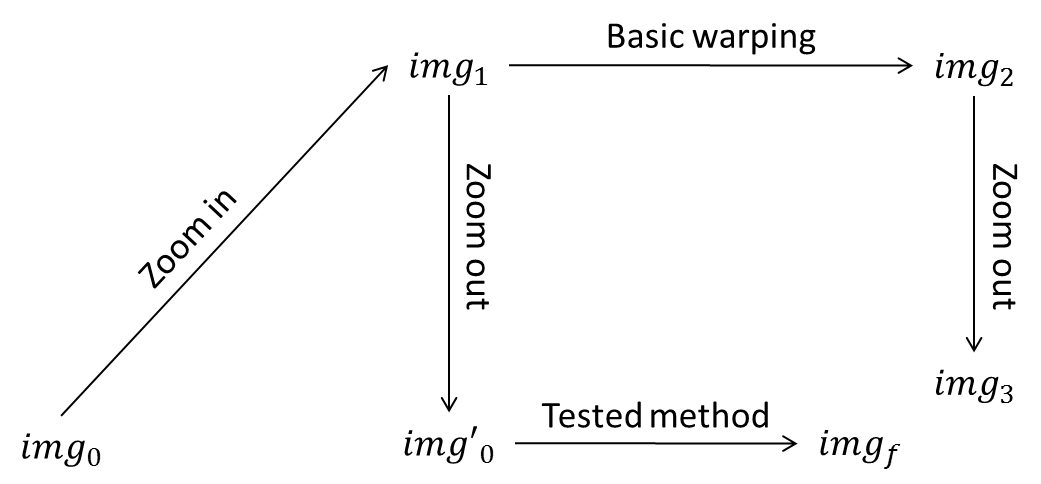
\includegraphics[width=0.8\textwidth]{SchemaGroundTruth.png}
\caption{Construction of the comparison with ground truth. $img_3$ is the ground truth, $img_f$ is the result of the tested algorithm.}
\label{SchemaGroundTruth}
\end{figure}
\begin{enumerate}
	\item Zoom in by a high factor an image $img_0$ (e.g. zoom in by a factor $10$) using zero-padding. The result is a huge and highly blurred image $img_1$.
	\item Zoom out $img_1$ using a Gaussian convolution to obtain an image $img_0'$ with same dimension than $img_0$.
	\item Resample $img_1$ by an homography mapping $H'$, to obtain an huge and blurred warped image $img_2$. The resampling method in this step does not matter a lot if the zoom factor is high enough and if the zoom out method prevents aliasing. Here a bilinear interpolation has been used.
	\item Zoom out $img_2$ using the same Gaussian convolution than in step 2 to obtain $img_3$. A perfect mapping method must warp $img_0'$ to $img_3$.
	\item Use the tested method to resample $img_0'$ by an homography mapping $H$. The result is a warped image $img_f$. The closer $img_f$ is to $img_3$, the better the method.
\end{enumerate}

\begin{remarques}
	\begin{itemize}
		\item $H'$ depends on $H$ and the zoom factor. $H'$ is obtained by conjugating (in the sense of matrice conjugation) $H$ by the dilatation matrix corresponding to the zoom out
		\item If $img_0'$ and $img_0$ have the same dimensions, and $img_f$ and $img_3$ have the same dimensions, but the size of $img_0'$ and $img_f$ can be different. However the Gaussian kernel must be the same (same standard deviation) because the ratio between $img_1$ and $img_0'$ is the same than the ratio between $img_2$ and $img_3$.
		\item $img_0'$ is a blurred but non-aliased version of $img_0$. Thus any aliasing appearing on $img_f$ has been introduced by the tested method. Moreover, since the Gaussian kernel to obtain $img_0'$ and $img_3$, overblurring will also be detected when comparing $img_f$ to $img_3$. Thus $img_3$ is the ground truth, i.e. the perfectly warped image from $img_0'$.
		\item The perfect mapping cannot be achieved from any $img_0$ only because the map $Z : img_1 \xrightarrow[]{\text{Zoom out}} img_0'$ is not inversible. If inversion is possible, then one just need to apply $Z^{-1}H'Z$ to any $img_0$ to perfectly compute any homography mapping. Thus here we take the problem from the other side : we start from a blurred $img_1$ and apply $Z$ to obtain an image $img_0'$, on which we already know $Z^{-1}$.
	\end{itemize}
\end{remarques}

The visual results correspond to figure \ref{VisualComparisonDecRipGrd}.

\begin{figure}
\centering
\subfigure[Geometric decomposition]{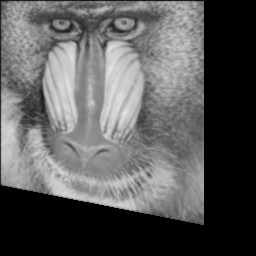
\includegraphics[width=0.4\textwidth]{img_num_dec.png}}
\subfigure[Ripmap]{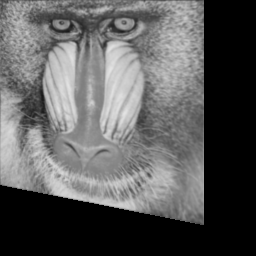
\includegraphics[width=0.4\textwidth]{img_num_rip.png}}
\subfigure[Ground Truth]{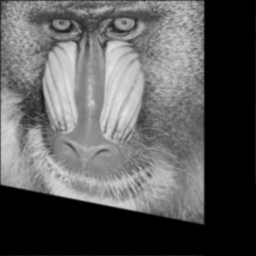
\includegraphics[width=0.4\textwidth]{img_num_grd.png}}
\caption{Visual comparison of the geometric decomposition, the ripmap and the ground truth}
\label{VisualComparisonDecRipGrd}
\end{figure}

The $L^1$- and $L^2$-norm of the error $|img_f-img_3|$ is given figure \ref{NumericalComparisonDecRipGrd}

\begin{figure}
\centering
\begin{tabular}{|c|c|c|}
\hline
Method & $L^1$ error  & $L^2$ error\\
\hline
Geometric decomposition & $\bf{0.44}$ & $\bf{0.64}$\\
\hline
Ripmap & 1.36 & 2.05\\
\hline
\end{tabular}
\caption{Numerical comparison between the Ripmap and the geometric decomposition. The ground truth is taken to compute the error to ideal. With the notation of figure \ref{SchemaGroundTruth}, the displayed quantities are The $L^1$- and $L^2$-norm of $|img_f-img_3|$}
\label{NumericalComparisonDecRipGrd}
\end{figure}